\documentclass[UTF8,fontset=fandol,11pt,a4paper]{ctexart}
\usepackage[a4paper,margin=1.75cm,headheight=15pt]{geometry}
\usepackage{amsmath,amssymb,mathtools,booktabs,tabularx,array,enumitem}
\usepackage[most]{tcolorbox}\usepackage{tikz}\usetikzlibrary{arrows.meta,positioning,calc}
\usepackage{xcolor,fancyhdr,hyperref,microtype,lastpage}
\newcolumntype{Y}{>{\raggedright\arraybackslash}X}\newcolumntype{L}[1]{>{\raggedright\arraybackslash}p{#1}}\newcolumntype{C}[1]{>{\centering\arraybackslash}p{#1}}
\setlength{\parindent}{2em}\setlength{\parskip}{0.34em}\setlength{\emergencystretch}{3em}\renewcommand{\arraystretch}{1.2}\setlength{\tabcolsep}{3pt}
\setlist[itemize]{itemsep=0.18em,topsep=0.35em,leftmargin=2em}\setlist[enumerate]{itemsep=0.18em,topsep=0.35em,leftmargin=2em}
\definecolor{deep}{RGB}{38,58,72}\definecolor{soft}{RGB}{244,247,248}\definecolor{greenish}{RGB}{52,91,74}\definecolor{warnc}{RGB}{136,61,58}\definecolor{purple}{RGB}{84,72,112}\definecolor{rulegray}{RGB}{110,116,120}
\hypersetup{colorlinks=true,linkcolor=deep,urlcolor=purple,pdftitle={CO-06 Cache 与存储层次}}
\pagestyle{fancy}\fancyhf{}\lhead{\small\color{deep}\textbf{408 · 计算机组成原理 CO-06}}\rhead{\small\color{deep}Locality · Identity · State · Cost}\cfoot{\small 第 \thepage\ 页 / 共 \pageref{LastPage} 页}\renewcommand{\headrulewidth}{0.4pt}
\newtcolorbox{corebox}[1]{breakable,colback=soft,colframe=deep,title=\textbf{#1},boxrule=0.8pt,arc=2mm}
\newtcolorbox{methodbox}[1]{breakable,colback=white,colframe=greenish,title=\textbf{#1},boxrule=0.7pt,arc=1.5mm}
\newtcolorbox{warnbox}[1]{breakable,colback=white,colframe=warnc,title=\textbf{#1},boxrule=0.7pt,arc=1.5mm}
\newtcolorbox{examplebox}[1]{breakable,colback=white,colframe=purple,title=\textbf{#1},boxrule=0.7pt,arc=1.5mm}
\newcommand{\kw}[1]{\textbf{\color{deep}#1}}\newcommand{\code}[1]{\texttt{#1}}
\tikzset{co/.style={draw=deep,rounded corners=1.5mm,text width=2.45cm,minimum height=0.95cm,align=center,fill=soft,font=\small,inner sep=3pt},state/.style={co,double,double distance=1.2pt,fill=white},flow/.style={-{Latex[length=2mm]},thick,draw=deep},fault/.style={co,draw=warnc,fill=white},ref/.style={-{Latex[length=2mm]},dashed,draw=rulegray}}
\title{\vspace{-1.1cm}\textbf{Cache 与存储层次}\\[0.4em]\large 怎样维护一个正确的高速副本，并把命中/缺失变成可靠的性能模型}
\author{408 · 计算机组成原理 Topic CO-06}\date{}

\begin{document}\maketitle

\begin{corebox}{母问题：小而快的副本怎样既保证“取对数据”，又真正降低平均访问成本？}
Cache 的知识不是若干并列名词，而是一条生成链：
\[
\boxed{
\begin{aligned}
\text{Locality}
&\to\text{Block Transfer}\to\text{Placement}\\
&\to\text{Identity / State}\to\text{Hit or Miss}\\
&\to\text{Replacement / Write}\to\text{Hierarchy Cost}
\end{aligned}}
\]
这些箭头表示\textbf{解释依赖}：局部性说明为什么值得保存副本；块搬运决定副本粒度；映射给出候选位置；tag/valid 等状态证明身份；只有状态轨迹确定后，命中率与 AMAT 才有可靠输入。
\end{corebox}

\begin{methodbox}{本册负责什么}
\begin{itemize}
\item \kw{Own：}block/line、set/way、tag/index/offset、hit/miss、3C、replacement、write-through/write-back、write-allocate/no-write-allocate、Cache 物理位数、local/global miss rate 与 AMAT。
\item \kw{Use：}CO-05 提供下一级主存/总线服务时间；CO-07 提供翻译后的地址与权限；CO-04 决定 miss 是否真的形成流水线 stall。
\item \kw{Stop Boundary：}页表、TLB page walk 与 fault 修复不在本册重新定义；OS Page Cache 也不是 CPU Cache 的同一个状态机。
\end{itemize}
\end{methodbox}

\tableofcontents\newpage

\section{为什么需要层次：单一介质同时满足不了速度、容量与成本}
存储系统同时追求更低延迟、更大容量和更低每位成本。寄存器、SRAM Cache、主存（408 中通常由 DRAM 实现）与后备存储在这些轴上取舍不同，因此系统利用局部性把近期更可能使用的信息保留在更近的层。

\kw{时间局部性}表示近期访问对象可能再次被访问；\kw{空间局部性}表示附近地址可能很快被访问。局部性只回答“为什么缓存可能有收益”，不证明某次访问一定命中。实际命中率还取决于块大小、容量、映射、相联度、替换策略和访问序列。

寄存器位于存储阶梯最上方，但由指令显式命名，不经过 Cache 式 placement/tag/replacement，因此不能机械当作又一级 Cache。

\section{对象与状态：先知道 Cache 到底保存什么}
\begin{methodbox}{核心对象}
\begin{itemize}
\item \kw{Block / Cache line：}Cache 与下一级之间搬运的数据粒度；line 是 Cache 中承载一个 block 副本的位置。
\item \kw{Set / Way：}set 是一次查找的候选集合；way 是组内的一条候选 line。
\item \kw{Tag：}证明候选 line 对应哪个下一级 block 的身份字段。
\item \kw{Valid：}说明当前 line 是否包含可用副本；tag 相同但 valid=0 仍不能命中。
\item \kw{Dirty：}write-back 下说明 Cache 副本比下一级更新，逐出前可能需要写回。
\item \kw{Replacement state：}组内 victim 选择所需的历史/近似状态；具体编码依实现与题设。
\item \kw{Pending / ready：}综合时序题中，miss 请求是否在途、返回数据何时可用；是否需要这类状态由题设决定。
\end{itemize}
\end{methodbox}

\subsection{地址字段：定位候选与定位块内字节}
设主存地址宽度为 $A$ 位，Cache 数据容量为 $C$ 字节，块大小为 $B=2^b$ 字节，相联度为 $E$，则组数
\[
S=\frac{C}{B E},\qquad s=\log_2S,
\]
字节编址时
\[
offset=b,\qquad index=s,\qquad tag=A-b-s.
\]
若题目按字编址，必须先把“块大小”换成每块包含多少个\textbf{编址单元}，不能直接沿用字节偏移位数。

地址字段属于\textbf{请求}；Cache line 中保存的是 data 与 metadata。index/offset 并不是每一行都重复存储的字段。

\subsection{数据容量与物理总位数}
若共有 $N_{lines}$ 条 line，则数据区位数为
\[
C_{data}=N_{lines}\times B\times 8.
\]
物理实现还可能包含 tag、valid、dirty、replacement、ECC 等：
\[
C_{physical}=\sum_{line}(data+tag+valid+dirty+metadata).
\]
题目说“Cache 容量”时先确认是 data-only，还是要求总物理位数。

\section{三类映射：先找候选，再证明身份}
\begin{center}\small
\begin{tabularx}{\linewidth}{L{2.2cm}L{2.2cm}YY}
\toprule
组织 & 候选范围 & 主要收益 & 主要代价\\\midrule
直接映射 & 每组 1 条 line & 查找和选择简单 & 冲突风险高\\
$E$ 路组相联 & 同组 $E$ 条 line & 冲突与硬件成本折中 & 多 tag 比较、victim 选择\\
全相联 & 全部 line & 映射冲突最少 & 比较器、功耗和替换成本最高\\
\bottomrule
\end{tabularx}
\end{center}

直接映射常写
\[
set=block\ number\bmod S.
\]
组相联先由 index 定位一组，再并行/逻辑上比较组内候选 tag；全相联不需要 set index。相联度增大通常能减少 conflict miss，但也可能增加比较器、功耗和 hit path 延迟，不能只说“越大越好”。

\begin{center}
\begin{tikzpicture}[node distance=0.72cm]
\node[co] (addr) {Request Address\\block / set / tag / offset};
\node[co,right=of addr] (cand) {Candidate Set\\由 index 定位};
\node[co,right=of cand] (id) {Identity Check\\valid + tag};
\node[co,right=of id] (data) {Block Data\\offset 选目标};
\draw[flow] (addr)--(cand);\draw[flow] (cand)--(id);\draw[flow] (id)--(data);
\end{tikzpicture}
\end{center}
上图箭头表示\textbf{查找依赖}，不是要求实现必须四拍串行；现代 Cache 可以并行读取 tag/data，但逻辑上仍要同时满足候选位置、身份有效和块内定位三个条件。

\section{Hit/Miss 生命周期：Cache 是状态机，不是命中率公式}
\subsection{Read hit}
定位候选组后，存在一条 line 同时满足 valid=1 且 tag 匹配，再用 offset 选出目标字节/字。命中只证明“本层已有可用目标副本”，不表示下一级没有副本，也不等价于地址翻译成功。

\subsection{Read miss}
最小生命周期为
\[
\begin{aligned}
\text{detect miss}
&\to\text{choose invalid/victim}
\to\text{write back if dirty}\\
&\to\text{fetch block}
\to\text{fill data/tag/state}
\to\text{retry or complete}.
\end{aligned}
\]
如果存在 invalid line，通常可直接使用；若必须逐出 victim，write-back Cache 还要检查 dirty。非阻塞 Cache、critical-word-first、MSHR 等只有题设明确时才加入；它们改变时序和重叠，不改变副本身份要求。

\begin{center}
\begin{tikzpicture}[node distance=0.65cm]
\node[co] (lookup) {Lookup\\set + valid/tag};
\node[co,right=of lookup] (hit) {Hit\\return data};
\node[fault,below=of hit] (miss) {Miss\\select line};
\node[co,right=of miss] (wb) {Dirty victim?\\必要时 write-back};
\node[co,right=of wb] (fill) {Lower level\\fetch + fill};
\node[co,right=of fill] (retry) {Retry / Complete};
\draw[flow] (lookup)--node[above,font=\scriptsize]{match}(hit);
\draw[flow] (lookup)|-node[left,font=\scriptsize]{no match}(miss);
\draw[flow] (miss)--(wb);\draw[flow] (wb)--(fill);\draw[flow] (fill)--(retry);
\end{tikzpicture}
\end{center}
这张图表示\textbf{状态转移与慢路径责任}；具体实现可重叠某些阶段。

\section{写策略：传播时机与写 Miss 行为是两条独立轴}
命中时：
\begin{itemize}
\item \kw{write-through：}同时更新下一级，状态关系直接，但写流量较大；
\item \kw{write-back：}先只更新 Cache 并置 dirty，逐出时才写回，降低平均写流量但增加状态与逐出成本。
\end{itemize}
写 miss 时：
\begin{itemize}
\item \kw{write-allocate：}先把目标 block 取入 Cache，再在本层修改；
\item \kw{no-write-allocate：}不为这次写分配 Cache line，写请求直接向下传播。
\end{itemize}
常见搭配不是逻辑必然。write-back 不自动推出 write-allocate，做题必须分别判断。

\begin{methodbox}{写缓冲的边界}
write-through 若要求 CPU 等每次下一级写完成，会直接暴露慢层延迟。write buffer 把待写请求先排入有限队列，在缓冲未满时允许前端继续；write-back 的 dirty victim 也可能进入 write-back buffer。二者都用队列吸收短时突发，但没有创造下一级长期带宽：若到达率持续高于排空率，最终仍会反压前端。
\end{methodbox}

\section{替换、3C 与反事实基线}
直接映射没有 victim 选择；组相联/全相联可使用 FIFO、Random、LRU 或近似策略。精确 LRU 的元数据与更新逻辑随相联度和编码方案变化，不能统一断言“每行只需要 $\log_2E$ 位”。

3C 分类必须绑定反事实基线：
\begin{itemize}
\item \kw{Compulsory miss：}该 block 第一次进入当前考察层；
\item \kw{Capacity miss：}即使换成同容量全相联基线，工作集仍装不下导致的 miss；
\item \kw{Conflict miss：}有限映射相对同容量全相联基线额外产生的 miss。
\end{itemize}
块大小、容量和访问序列改变后，分类结果也可能改变。

在\textbf{同一引用串、全相联且采用栈算法（如经典 LRU）}的模型中，增大容量不会增加 miss 数；Belady anomaly 是非栈策略可能出现的性质。这个结论不能越过“全相联/同一引用串/策略”条件直接套到任意 Cache 组织。

\section{性能语言：先定义路径，再算 AMAT}
\subsection{先分清时间和速率}
\kw{Latency} 是一般的请求到结果可用等待；\kw{Access Time} 是某存储器件/接口完成规定访问的时间；\kw{Cycle Time} 强调同一资源下一次合法启动操作的间隔。\kw{Throughput} 是单位时间完成的请求/事务数，\kw{Bandwidth} 是单位时间传输的有效数据量。多体交叉和 burst 常主要提高吞吐量/带宽，并不保证单次访问 latency 同比例下降。

\subsection{Hit Time、Miss Total Time 与 Miss Penalty}
若当前层 hit 路径总时间为 $T_{hit}$，miss 从原请求开始到最终完成的总时间为 $T_{miss,total}$，本册规范化定义
\[
MP=T_{miss,total}-T_{hit},
\]
即 miss penalty 是\textbf{相对 hit 的额外成本}。若题面“缺失损失 200 cycles”未说明是额外代价还是完整 miss path，不要擅自把它记作 $MP$；先保留 $T_{miss,total}$ 再由题意判断。

\subsection{AMAT 是路径时间的期望}
若 hit rate 为 $HR$、miss rate 为 $MR=1-HR$，则定义式为
\[
AMAT=HR\,T_{hit}+MR\,T_{miss,total}.
\]
在上面的 $MP$ 定义下才可化简为
\[
\boxed{AMAT=T_{hit}+MR\times MP}.
\]
它不是第二条独立公式，而是条件期望的代数化简。

\begin{center}
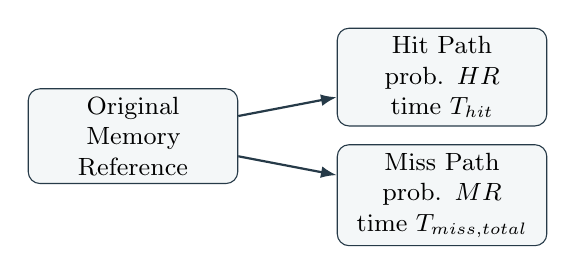
\begin{tikzpicture}[node distance=1.0cm]
\node[co] (req) {Original\\Memory Reference};
\node[co,right=1.25cm of req,yshift=0.75cm] (h) {Hit Path\\prob. $HR$\\time $T_{hit}$};
\node[co,right=1.25cm of req,yshift=-0.75cm] (m) {Miss Path\\prob. $MR$\\time $T_{miss,total}$};
\draw[flow] (req)--(h);\draw[flow] (req)--(m);
\node[right=0.65cm of req,font=\small] at ($(req.east)+(2.7cm,0)$) {};
\end{tikzpicture}
\end{center}
图中的分支是\textbf{互斥完成路径}；真实硬件是否并行、重叠，要先画事件时间线再决定 $T_{hit}$ 和 $T_{miss,total}$ 包含什么。

\subsection{多级 Cache：只有走到下一层才支付下一层成本}
若 L1 hit time 为 $t_1$、local miss rate 为 $m_1$；L2 被访问后的 hit time 为 $t_2$、local miss rate 为 $m_2$；L2 miss 后主存服务时间为 $t_M$，并暂不考虑额外写回/重叠，则
\[
AMAT_{L1}=t_1+m_1\left(t_2+m_2t_M\right)
=t_1+m_1t_2+m_1m_2t_M.
\]
L2 的 \kw{local miss rate} 以实际到达 L2 的请求为分母；\kw{global miss rate} 以 CPU 原始 references 为分母。在“每个 L1 miss 恰好访问一次 L2、无 bypass/prefetch 额外请求”的简单模型中，L2 global miss rate 为 $m_1m_2$。

下一级 AMAT、脏 victim 写回、总线仲裁、refill 与 retry 都可能进入上一级 miss path。若题设允许 non-blocking Cache、write buffer、prefetch 或流水线隐藏部分等待，某些时间可能相加、取最大，或根本不形成 CPU stall。\kw{AMAT 是每个 memory reference 的接口平均成本，不等于整个程序的 CPU time。}

\section{地址翻译接口：翻译层次、数据层次和虚存慢路径不是一条链}
PIPT、VIPT、VIVT 是 Cache 与地址翻译的接口组织：PIPT 等翻译得到 PA 后查 Cache；VIPT 可用页内偏移中的 index 与 TLB 并行，再用翻译后的物理 tag 确认身份；VIVT 则需要处理 synonym/homonym 等额外一致性问题。

若 page offset 为 $p$ 位、block offset 为 $b$ 位，VIPT 在经典约束下可用于 set index 的位数至多为 $p-b$，等价写成
\[
sets\times block\ size\le page\ size.
\]
这个限制来自“index 必须完全落在翻译不改变的 page offset 中”，不是固定容量口诀。

\begin{center}
\begin{tikzpicture}[node distance=0.58cm]
\node[co] (va) {CPU Request\\Virtual Address};
\node[co,right=of va] (tr) {Translation Track\\TLB / Page Walk};
\node[co,right=of tr] (pa) {Legal PA\\+ permission};
\node[co,right=of pa] (cache) {Data Track\\L1/L2/LLC/主存};
\node[fault,below=0.9cm of tr] (pf) {Fault Track\\OS repair / reject};
\draw[flow] (va)--(tr);\draw[flow] (tr)--(pa);\draw[flow] (pa)--(cache);\draw[flow] (tr)--(pf);
\draw[ref] (pf)-|node[below,font=\scriptsize]{修复后 retry}(va);
\end{tikzpicture}
\end{center}
上图箭头表示\textbf{语义依赖与控制转移}。不能把它压成无条件的 `TLB → L1 → L2 → 主存 → 磁盘`：TLB 缓存翻译，Cache 缓存数据块，页面不驻留时才进入 OS 的 fault 慢路径。

\section{贯穿母例：两个块反复映射到同一组}
设直接映射 Cache 有 $S$ 组、块大小 $B$，两个主存块 $x$ 与 $y$ 满足
\[
x\bmod S=y\bmod S,\qquad x\neq y.
\]
它们交替访问时都会定位同一条候选 line，但 tag 不同，因此可能反复互相驱逐。这个例子同时验证：
\begin{enumerate}
\item index 只负责定位候选，不证明身份；
\item tag/valid 才决定 hit；
\item 直接映射冲突来自 placement 约束，而不是 Cache 其余空间真的已满；
\item 提高相联度可允许两块在同组共存，但会增加比较和替换成本；
\item 命中率变化最终还要连同 hit time 与 miss penalty 才能判断性能收益。
\end{enumerate}

\section{概念边界：相似词必须改变做题行为}
\begin{center}\small
\begin{tabularx}{\linewidth}{L{2.2cm}L{2.8cm}YY}
\toprule
边界 & 为什么容易混淆 & 真正判据 / 题面信号 & 混淆后果\\\midrule
地址字段 $\neq$ line 内容 & 都出现 tag/index/offset & 请求字段用于定位；line 只保存 data+metadata & 错算物理容量\\
Hit rate $\neq$ Performance & 命中高常常更快 & 还需 hit time、penalty、写流量与重叠 & 只凭命中率判快慢\\
Miss penalty $\neq$ Miss total time & 都会被叫“缺失时间” & 前者是额外成本；后者含当前层查找 & 重复或漏算 hit time\\
Local MR $\neq$ Global MR & 都写 miss rate & 分母是本层 accesses 还是 CPU refs & 多乘/少乘上层 miss rate\\
Write-back $\neq$ Write-allocate & 常作为搭配出现 & 一个管命中后的传播，一个管写 miss 是否取块 & 从一轴错误推出另一轴\\
Conflict $\neq$ Capacity & 都会逐出 line & 同容量全相联反事实基线是否仍 miss & 选错优化方向\\
Latency $\neq$ Bandwidth & 都描述“快” & 单请求等待 vs 单位时间数据量 & 用带宽推出随机访问延迟\\
Cache miss $\neq$ Page Fault & 都进入慢路径 & 数据块副本缺失 vs 翻译/驻留/权限 fault & 把硬件 miss 写成 OS 调页\\
\bottomrule
\end{tabularx}
\end{center}

\section{做题控制协议：从请求到成本只走一次}
\begin{enumerate}
\item \kw{Reference：}先确认题目统计哪些 instruction/data references，一条源语句可能产生多次访问；
\item \kw{Granularity：}统一编址单位、block size、Cache data size、set/way；
\item \kw{Address：}求 block/set/tag/offset，不把地址字段写进 line metadata；
\item \kw{State：}逐次维护 valid/tag/dirty/replacement；
\item \kw{Lifecycle：}miss 时写 victim、write-back、lower-level fetch、fill、retry；写 miss 再判断 allocate；
\item \kw{Count：}先数 hit、miss、write-back、lower-level transactions；
\item \kw{Cost：}声明 hit time、miss total / extra penalty、local/global miss rate 和重叠；
\item \kw{Verify：}检查访问总数、块数上界、概率范围、地址位数和独立时间口径。
\end{enumerate}

\begin{methodbox}{陌生题第一动作}
先问两句话：\kw{“当前请求对应哪个 block/set/tag/offset？”“当前 line 的身份与状态是否足以证明这是目标副本？”} 只有这两问闭合后，才进入命中率和 AMAT。
\end{methodbox}

\section{本册与其他 Owner 的接口}
\begin{center}\small
\begin{tabularx}{\linewidth}{L{3cm}YY}
\toprule
相邻 Owner & 本册使用什么 & 什么时候停止本册\\\midrule
CO-05 主存与存储硬件 & 下一级 latency、burst、bank、bandwidth & 开始推 DRAM/总线事务内部细节\\
CO-07 地址翻译 & 合法 PA、permission、PIPT/VIPT 条件 & 开始推 VPN/PFN、page walk、TLB 状态\\
CO-04 流水线 & miss stall / overlap 边界 & 开始问哪条指令何时 ready/commit\\
OS-04 / X-B02 & Page Fault 后的 repair/retry 结果 & 开始分配 frame、page-in、COW、replacement\\
\bottomrule
\end{tabularx}
\end{center}

\begin{corebox}{一页压缩}
Cache 先解决\textbf{正确副本}，再讨论\textbf{平均性能}：
\[
\boxed{
\begin{aligned}
\text{Reference}
&\to\text{Block/Set/Tag/Offset}
\to\text{Valid Identity Check}\\
&\to\text{Hit or Miss State Transition}
\to\text{Event Count}
\to\text{Path Cost / AMAT}
\end{aligned}}
\]
忘掉具体公式时，从“候选位置 + 身份 + 状态 + 慢路径 + 路径期望”即可重新生成主要结论。
\end{corebox}

\end{document}
